\section{Dinaminių puslapių peržiūros problema}

Saityno peržvalgos robotų sistemų tradicinis modelis remiasi HTTP užklausomis į konkretų žiniatinklio serverį, kurį identifikuoja URL adresas. Taigi, tradicinės tokių sistemų implementacijos darydavo prielaidą, jog URL adresas unikaliai identifikuoja statinį turinį žiniatinklyje. Šis požiūris tapo nebetinkamas, kai W3C konsorciumas standartizavo AJAX\footnote{AJAX - Asynchronous JavaScript and XML} formatą asinchroninei žiniatinklio kliento komunikacijai su serveriu \cite{AJAXCrawlResearch}. Išplito dinaminiai puslapiai, kurie savo turinio dalis keičia asinchroniškai bendraudami su serveriu ir apsikeisdami informacija. Ši problema tapo itin aktuali su Vieno puslapio aplikacijų \footnote{SPA - Single Page Applications} ir jų kūrimo karkasų, tokių kaip React, Angular ar VueJS išpopuliarėjimu. Šiame skyriuje palyginamas tradicinis žiniatinklio resursų modelis su nauju, AJAX technologija grįstu modeliu, apžvelgiamos rinkoje taikomos praktikos naujo tipo žiniatinklio programų žvalgymui.

\subsection{Tradicinis žiniatinklio programos modelis}

Tradicinis žiniatinklio programos modelis remiasi sinchronine kliento-serverio komunikacija, kurioje klientas neturi jokios verslo logikos, visa puslapio žymėjimo ir stiliaus kodo sukonstravimo logika vyksta serverio pusėje. Tokiame modelyje saityno serveriai apkraunami tinklo užklausomis, nes norint pakeisti ar atnaujinti bet kokią puslapio dalį, reikalinga perkrauti visą puslapį iš naujo -- nusiųsti pakartotinę HTTP užklausą serveriui. Supaprastinta tokio modelio schema pateikiama \ref{fig:traditional_web_model} paveikslėlyje. 

\begin{figure}[htp!]
\centering
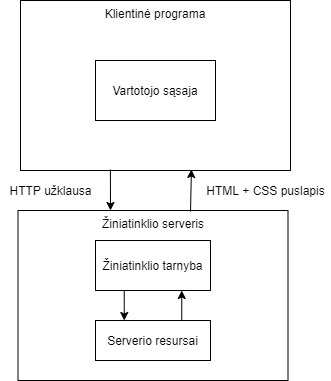
\includegraphics[scale=0.6]{img/Traditional_Web_Model.png}
\caption{Tradicinis žiniatinklio svetainės komunikacijos modelis \cite{AJAXCrawlResearch}}
\label{fig:traditional_web_model}
\end{figure}

Pagrindiniai tokio modelio trūkumai:
\begin{itemize}
    \item Visa kodo vykdymo logika atliekama serveryje
    \item Pakartotinis dublikuotų duomenų perdavimas
    \item Ganėtinai lėti serverio atsako laikai dėl pilno resurso užklausimo
\end{itemize}

\subsection{AJAX žiniatinklio programos modelis}

AJAX modelis taikomas naujo tipo vieno puslapio žiniatinklio svetainėse, kurių pagrindinis bruožas -- būsena kliento pusėje ir jos atnaujinimas dinamiškai reaguojant į kliento įvykius (angl. -- \textit{DOM Events}) ir siunčiant asinchronines AJAX užklausas į serverį. Detalesnė tokio modelio schema pateikiama \begin{figure}[htp!]
\centering
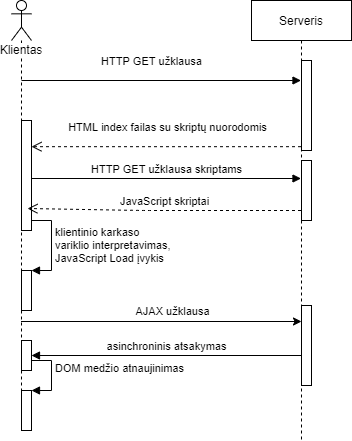
\includegraphics[scale=0.7]{img/csr.png}
\caption{Kliento pusės atvaizdavimas \cite{JavaScriptCrawl}}
\label{fig:csr}
\end{figure} paveikslėlyje.

\subsubsection{AJAX modelio žvalgymo problema}

Tradiciniai žvalgymo robotai keliauja žiniatinklio grafu vykdydami HTTP GET užklausas, išgaudami nuorodas tiesiai iš serverio grąžinamo HTML kodo. Naujojo AJAX modelio svetainės reikalauja, jog svetainė būtų užkraunama pilnai, t.y. atsiunčiamas ir įvykdomas JavaScript kodas. Kitaip tariant, paieškos žvalgymo robotas turi elgtis panašiai kaip paprastas naršykle besinaudojantis žmogus \cite{JavaScriptCrawl}.

\subsubsubsection{„Googlebot“ taikoma praktika žvalgant AJAX svetaines}

„Googlebot“ žvalgymo robotas paiešką atlieka 3 etapais:
\pagebreak

\begin{enumerate}
    \item Žvalgymas (angl. -- \textit{Crawling})
    \item Atvaizdavimas (angl. -- \textit{Rendering})
    \item Indeksavimas
\end{enumerate}

Atvaizdavimo etapas atliekamas būtent AJAX tipo dinaminėms svetainėms, kaip skelbiama „Google“, šiam procesui naudojama atvaizdavimo eilė, iš kurios agentai žinutes paima tuomet, kai atsilaisvina „Google“ žvalgymo infrastruktūros resursai. Tipiškai tai gali užtrukti nuo kelių minučių iki kelių savaičių. Išsamesnė „Googlebot“ žvalgymo ir atvaizdavimo (angl. -- \textit{Rendering}) schema pavaizduota \ref{fig:googlebot_rendering} paveikslėlyje.

\begin{figure}[htp!]
\centering
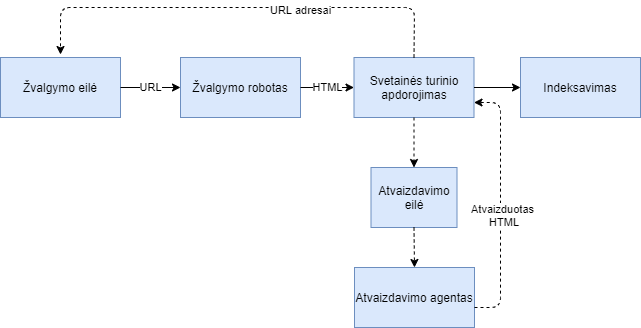
\includegraphics[scale=0.7]{img/Googlebot_rendering.png}
\caption{„Googlebot“ žvalgymo procesas \cite{GooglebotCrawling}}
\label{fig:googlebot_rendering}
\end{figure}

Pavaizduotoje schemoje atvaizdavimo procese yra naudojamas „Chromium“ naršyklės variklis be vartotojo sąsajos, kuris sugeba įvykdyti svetainės JavaScript kodą. Tiesa, „Google“ neatskleidžia, koks roboto svetainės užkrovimo maksimalus laukimo laikotarpis. Kaip teigiama, kol kas „Chromium“ variklis yra leidžiamas atskirai nuo bendrų „Google Chrome“ naršyklės išleidimų, todėl jo funkcionalumai ir palaikomos ECMAScript naujovės atsilieka, todėl atvaizdavimo metu „Googlebot“ gali nesuprasti naujausių svetainės sintaksės elementų. \cite{GooglebotCrawling}.